\documentclass{article}
\usepackage[utf8]{inputenc}
\usepackage{graphicx}
\usepackage[section]{placeins}

\title{SocialIqa\_pt: A Translation of a Common-Sense Reasoning Dataset about Social Interactions}
\author{Fabio Grassiotto}
\date{30 June 2024}

\begin{document}

\maketitle

\begin{abstract}
    The objetive of this work is to create a Portuguese language translation of
    the English dataset Social IQa, a benchmark of 38,000 multiple choice
    questions for the evaluation of emotional and social intelligence in a
    number of everyday situations. The approach taken here was to perform
    machine translation using popular models available at Hugging Face, rank
    translations using a GPT-driven evaluation (GEMBA) and select the best for
    our dataset.
\end{abstract}

\section{Introduction}

Common-Sense inteligence, the human ability of applying practical knowledge for
decisions in everyday life, is still considered a challenging task for AI
systems. As it can be readily perceived when interacting with chatbots, these
systems lack the ability to, through intuition, reason about common situations
and events. It is clear that such reasoning requires background knowledge about
how the world works, incluind the rich nuanced interaction between people in the
social sphere. \cite{choi2022curious, krause2023commonsense}

Therefore, the availability of datasets capable of benchmarking AI systems on
this task is of utmost importance. Datasets such as Social IQa are readily
available in the english language, but we are not aware of any in portuguese.
\cite{sap2019socialiqa}

The portuguese language cannot be truly considered a low-resource language aas
it is the case with some of the African and Asian languages, as there are
datasets already available in portuguese that have millions of tokens, but there
are certainly gaps that should be addressed. \cite{ghafoor2021impact}

One of the gaps is certainly in the availability of datasets that deal with
common sense-reasoning and in special datasets that adress social interactions.

This work is structured as follows:
\begin{itemize}
    \item Section 1 \textbf{(this section)}: Here we introduce the work and its
    motivation.
    \item Section 2 \textbf{Methodology}: We describe the translation process
    and the evaluation system we employed.
    \item Section 3 \textbf{Dataset}: We describe the SocialIqa dataset in
    detail.
    \item Section 4 \textbf{Results} : We describe the translated sets results
    and compare them in detail.
    \item Section 5 \textbf{Conclusion and Future Works}: We analyse the results
    we achieved and describe next steps to be taken.
\end{itemize}

\section{Methodology} 

Our translation process consisted of the five steps described in Figure
\ref{fig:diagram} below. All steps are executed using Python notebook files
available at.

\begin{itemize}
    \item \textbf{Step I: English dataset conversion} In this step, the original
    english dataset was converted from JSON format into a temporary 
    comma-delimited file format for easier processing. The conversion was
    performed on file read\_dataset\_en.ipynb.
    \item \textbf{Step II: Machine Translation} In this step, the original
    dataset, available in three separate files for the development, training and
    testing sets, was translated to the portuguese language using three distinct
    models on files translator\_marian.ipynb, translator\_t5.ipynb and translator\_nllb.ipynb.
        \begin{itemize}
            \item Helsinki-NLP/opus-mt-tc-big-en-pt
            \item unicamp-dl/translation-en-pt-t5
            \item facebook/nllb-200-distilled-1.3B
        \end{itemize}
    \item \textbf{Step III: Translation Evaluation} Translations were evaluated
    using the evaluation metric GEMBA - GPT Estimation Metric Based Assessment
    \cite{kocmi2023large} using GPT3.5-turbo. To use the metric, the prompt was
    modified to not use human reference in the evaluation and to evaluate the
    translations of the three models of this work simultaneously 
    \item \textbf{Step IV: Translation selection and ranking} The highest ranked translation set
    was selected based on the metric described above and used in the dataset.
    The implementation for steps III and IV is executed on files
    evaluator\_gemba\_dev.ipynb, evaluator\_gemba\_train.ipynb and
    evaluator\_gemba\_tsyt.ipynb respectively for the development, training and
    test sets.
    \item \textbf{Step V: Portuguese Dataset publishing}  In this step, the
    comma-delimited file with the final translation contents was converted to
    JSONL format for publishing. The conversion was performed on file 
    publish\_dataset\_pt.ipynb.
\end{itemize}
 
\begin{figure}[htbp]
    \centering
    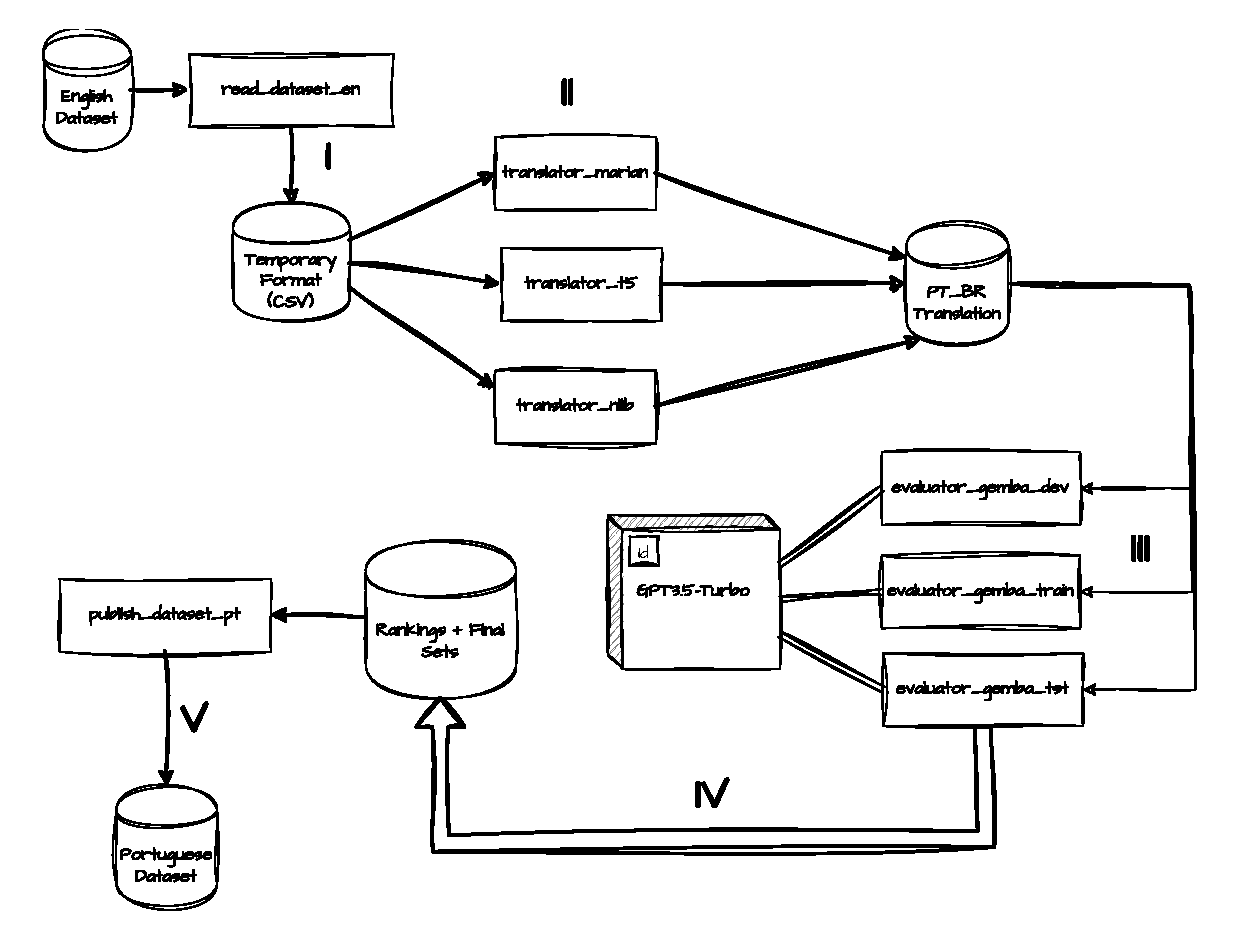
\includegraphics[width=1\textwidth]{drawio/translation.drawio.pdf}
    \caption{\label{fig:diagram}Translation process including machine
    translation and GPT-based evaluation to select the best possible
    translation.}
\end{figure}


\section{Dataset}

\section{Results}

\begin{figure}[htbp]
    \centering
    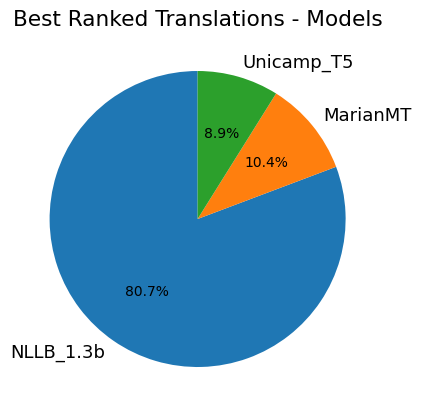
\includegraphics[width=0.5\textwidth]{figures/pie-chart.png}
    \caption{\label{fig:pie}Figure example.}
\end{figure}

\begin{figure}[htbp]
    \centering
    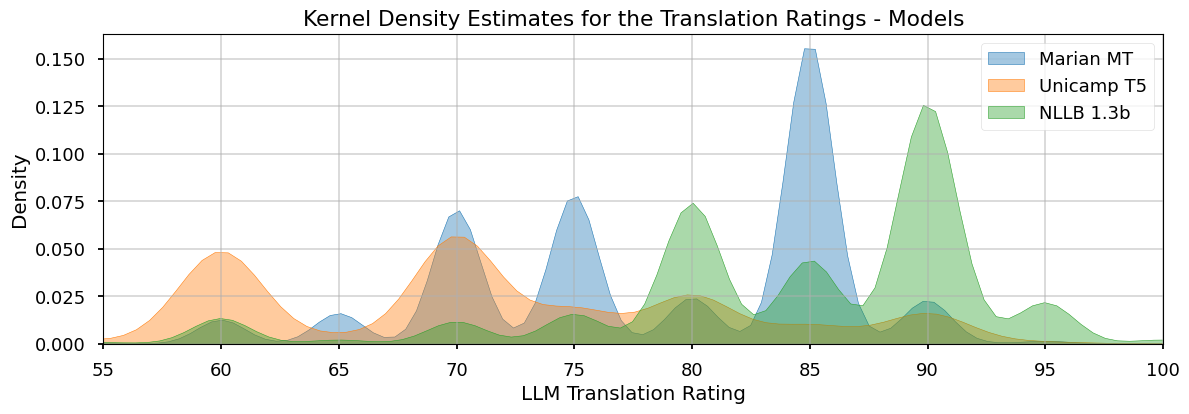
\includegraphics[width=1\textwidth]{figures/kde.png}
    \caption{\label{fig:kde}Figure example.}
\end{figure}

\begin{figure}[htpb]
    \centering
    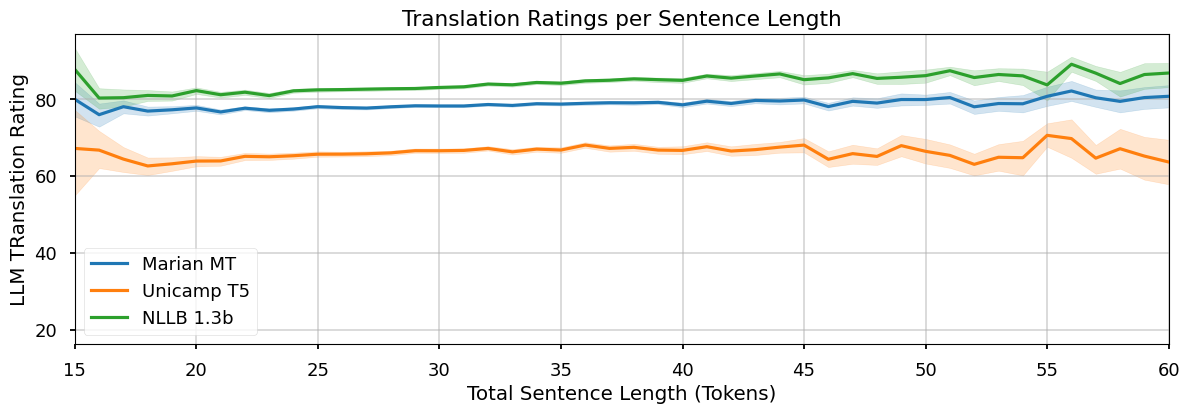
\includegraphics[width=1\textwidth]{figures/line-chart.png}
    \caption{\label{fig:line-chart}Figure example.}
\end{figure}

Figure~\ref{fig:pie} is an example of figure citation.

\section{Conclusion and Future Work}

% Usando a bibliografia com arquivo no formato bibtex, (ver arquivo main.bib que
% faz parte desse projeto)
\bibliographystyle{plain}
\bibliography{main.bib}

\end{document}
